\chapter{Metodología}\label{metodologia}

En esta sección repasaremos cómo hemos dividido y organizado las 300 horas de desarrollo del proyecto. Trataremos tanto las fases de preparación e introducción así como el desarrollo en sí y su verificación y repaso.

\section{Fases del desarrollo}

\begin{figure}[h]
    \centering
    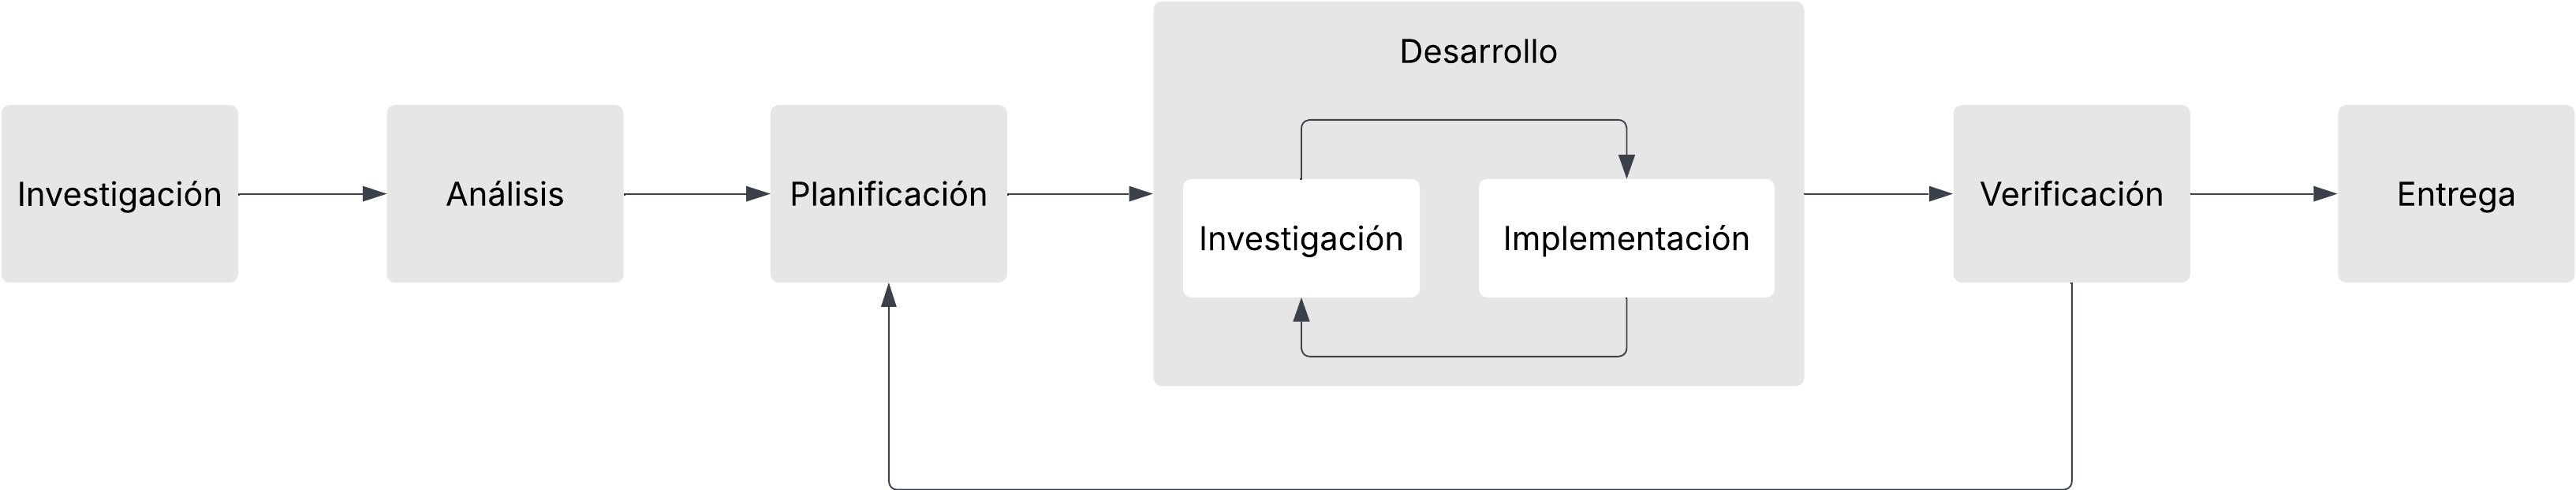
\includegraphics[width=1\linewidth]{img/metodologia.png}
    \caption{Fases del desarrollo}
    \label{fig:metodologia}
\end{figure}

\subsection{Investigación}

Dado que la criptografía post-cuántica en general, y SIKE con su base matemática en isogenias es un tema complejo que no habíamos tratado previamente, decidimos empezar investigando para comenzar el desarrollo con, al menos, una visión general del protocolo.

El artículo principal que hemos tratado ha sido la presentación de de Feo, Jao y Plût al NIST \cite{towards_quantum_resistant_cryptosystems}. Sin embargo, debido a la alta complejidad matemática, hemos tenido que dar varios rodeos antes de poder centrarnos en él y realmente interiorizarlo.

Algunos de los temas que hemos tenido que estudiar son curvas elípticas, sobre todo las consideradas supersingulares, isogenias y $j$-invariantes. Todos estos temas se ven reflejados en el capítulo \ref{conceptosprevios}, de Conceptos Previos.

\subsection{Análisis}

Una vez tuvimos una idea general del protocolo y de sus bases, nos sentimos ya preparados para hacer un primer esquema del qué y el cómo íbamos a hacer. Incluye tanto la realización de un primer esquema de la memoria como el de la interfaz gráfica.

Esta fase es la más corta ya que tan sólo consiste en una vista general de la organización, no una planificación concreta.

\subsection{Planificación}

Una vez definido el objetivo final general con una visión específica de qué había que redacar y/o implementar, desmigamos el proceso para comenzar el desarrollo del proyecto de una forma razonable y eficaz.

Durante este primer proceso de planificación, definimos las actividades principales así como sus componentes, en caso de considerarlo necesario. Se clasifican estas tareas por su dominio (memoria, frontend o backend) y por su prioridad (crítica, alta, media, baja y opcional).

La planificación no sólo se queda aquí, conforme empezamos a desarrollar, nos encontramos incidencias que debemos manejar. De esta forma el trío planificación-desarrollo-verificación forma un bucle sobre el que iteraremos a lo largo del desarrollo del proyecto.

\subsection{Desarrollo}

Durante la fase de desarrollo estamos trabajando en el proyecto de manera efectiva, ya sea escribiendo parte de la memoria o la implementación gráfica. Esta fase tiene sus propias fases internas de investigación y desarrollo/implementación de parte de la interfaz gráfica. En general hemos trabajado con tecnologías que conocíamos, sin embargo, siempre hay innovaciones y mejoras que debemos probar y verificar a lo largo de un proyecto software, por pequeño que sea.

\subsection{Verificación}

En esta fase, comprobamos que todo vaya correcto. Esto incluye revisiones por parte del tutor así como pruebas formales e informales de la interfaz gráfica. Durante esta fase anotamos todo aquello que no ha ido como debería para, volviendo a la fase de planificación, poder crear las nuevas actividades de manera rigurosa.

\subsection{Entrega}

La entrega es la fase final, una vez el proyecto terminado, se procede a la entrega oficial de la memoria y la realización de la presentación y la defensa del proyecto.